% LLNCStmpl.tex
% Template file to use for LLNCS papers prepared in LaTeX
%websites for more information: http://www.springer.com
%http://www.springer.com/lncs



\documentclass{llncs}
%Use this line instead if you want to use running heads (i.e. headers on each page):
%\documentclass[runningheads]{llncs}

\usepackage{qtree}
\usepackage{amsmath}
\usepackage{amsfonts}
\usepackage{graphicx}
\usepackage{algorithmicx}
 \usepackage{algpseudocode}
\usepackage{float}
\usepackage{wrapfig}
\usepackage{listings}

\usepackage{geometry}
\usepackage{listings}
\usepackage{color}
\usepackage[usenames,dvipsnames,svgnames,table]{xcolor}
%\geometry{a4paper}

\begin{document}
\title{Sentiment Analysis of Streaming Data}

%If you're using runningheads you can add an abreviated title for the running head on odd pages using the following
%\titlerunning{abreviated title goes here}
%and an alternative title for the table of contents:
%\toctitle{table of contents title}

\subtitle{Cloud Computing - Project Report}

%For a single author
%\author{Author Name}

%For multiple authors:
\author{Aditya Sapate\inst{1} \and Chaitanya Munukutla\inst{2}}


%If using runnningheads you can abbreviate the author name on even pages:
%\authorrunning{abbreviated author name}
%and you can change the author name in the table of contents
%\tocauthor{enhanced author name}

%For a single institute
%\institute{Institute Name \email{email address}}

% If authors are from different institutes 
\institute{IIT Madras \email{CS10B031} \and IIT Madras \email{CS10B040}}

%to remove your email just remove '\email{email address}'
% you can also remove the thanks footnote by removing '\thanks{Thank you to...}'


\maketitle

\section{Motivation}
Social Media has creeped into everybody's lives and pockets. Constant feeds about the things that we care about, make up today's \textbf{news streams}. But, the user prespective about a specific topic is still not taken under serious consideration. \\ \\ For example, a review of a recently released movie may be trending. But, it's not known whether it's trending on the positive or the negative light of user opinions. The current project aims at realtime sentiment analysis of social feeds, which serves the above purpose. THe case study uner consideration is the \emph{Twitter Stream}.

\section{Stream Processing}

The current project aims at steam processing the tweets in realtime, in contrast to tradiationl batch-processing systems. This has been achieved by using \textbf{Apache Storm}.

A Storm cluster is superficially similar to a Hadoop cluster. Whereas on Hadoop you run "MapReduce jobs", on Storm you run "topologies". "Jobs" and "topologies" themselves are very different -- one key difference is that a MapReduce job eventually finishes, whereas a topology processes messages forever (or until you kill it).

There are two kinds of nodes on a Storm cluster: the master node and the worker nodes. The master node runs a daemon called "Nimbus" that is similar to Hadoop's "JobTracker". Nimbus is responsible for distributing code around the cluster, assigning tasks to machines, and monitoring for failures.

Each worker node runs a daemon called the "Supervisor". The supervisor listens for work assigned to its machine and starts and stops worker processes as necessary based on what Nimbus has assigned to it. Each worker process executes a subset of a topology; a running topology consists of many worker processes spread across many machines.

Hence, in our current present situation, a stream of tweets form the input data, and the topology we build, distributes them among "Supervisor" nodes.

\subsection{Streams}
The core abstraction in Storm is the "stream". A stream is an unbounded sequence of tuples. Storm provides the primitives for transforming a stream into a new stream in a distributed and reliable way. For example, you may transform a stream of tweets into a stream of trending topics.

The basic primitives Storm provides for doing stream transformations are "spouts" and "bolts". Spouts and bolts have interfaces that you implement to run your application-specific logic.

A \textbf{spout} is a source of streams. A spout may connect to the Twitter API and emit a stream of tweets.

A \textbf{bolt} consumes any number of input streams, does some processing, and possibly emits new streams. Complex stream transformations, like computing a stream of trending topics from a stream of tweets, require multiple steps and thus multiple bolts. Bolts can do anything from run functions, filter tuples, do streaming aggregations, do streaming joins, talk to databases, and more. \\

Networks of spouts and bolts are packaged into a \textbf{topology} which is the top-level abstraction that you submit to Storm clusters for execution. A topology is a graph of stream transformations where each node is a spout or bolt. Edges in the graph indicate which bolts are subscribing to which streams. When a spout or bolt emits a tuple to a stream, it sends the tuple to every bolt that subscribed to that stream.

\subsection{Data Model}
Storm uses tuples as its data model. A tuple is a named list of values, and a field in a tuple can be an object of any type. Out of the box, Storm supports all the primitive types, strings, and byte arrays as tuple field values. To use an object of another type, you just need to implement a serializer for the type.

\subsection{Using Twitter4J to access Twitter API}
Twitter4J has been used to make the project talk to the Twitter API. Since, the Twitter is the input stream under consideration, the spout that collects the tweets is written using the twitter4j library.

\subsubsection{Authentication} 
The latest Twitter policy forced the creation of developer credentials so as to access public or private streams. So, the Twitter stream is pinged after authentication through OAuth.

\lstinputlisting[language=Java, firstline=4]{filterQuery.java}

\subsubsection{Filter Queries}
Instead of collecting random tweets from all over the world, we use filter queries, to retrieve tweets which satisfy our criterion, for example, movie and product reviews. This is given directly as an argument to the spout constructor.

\lstinputlisting[language=Java, firstline=1, lastline=2]{filterQuery.java}

Alternatively, we can also filter the tweets by their location.

\lstinputlisting[language=Java, firstline=9, lastline=12]{filterQuery.java}

Tweets can also be filtered by their input language.

\lstinputlisting[language=Java, firstline=3, lastline=3]{filterQuery.java}


\section{Sentiment Analysis}

\subsection{Peter D. Turney, \emph{Semantic Orientation Applied to Unsupervised Classification of Reviews}, 2002}

The above paper presented a simple unsupervised learning algorith  for classifying reviews as \emph{recommended}(thumbs up) or \emph{not recommended}(thumbs down)

\subsubsection{Extracting Phrases with Adjectives or Adverbs}
Replying on past work by Hatzivassiloglou and Wiebe (2000) which showed that adjectives and adverbs are good indicators of subjective, evaluative sentences, the algorithm first extracts all the phrases of the review which contain an adverb or an adjective.

However, procuring an isolated adjective may lead to different opinions in different contexts. For example, "unpredictable plot" may lead to a positive opinon under the context of a movie review, but "unpredictable steering" leads to a negative opinion under the context of an automotve review. So, the lone word "unpredictable" should not be relied on, and hence the current algorithm extracts two consecutive words, of which, the second word most usually depicts the situation or context of the review.

\subsubsection{Estimating the Semantic Orientation}
The estimation of semantic orientation of the extracted phrase uses the PMI-IR algorithm (Church and Hanks, 1989). The \textbf{Pointwise Mutual Information} between two words $word_1$ and $word_2$ can be defined as follows,
$$
PMI(word_1, word_2) = \log _2 \left( \dfrac{P(word_1 \ \& \ word_2)}{P(word_1) \bullet P(word_2)} \right)
$$

Here, $P(word_1 \ \& \ word_2)$ denotes the probability of the co-occurence of both $word_1$ and $word_2$.

The Semantic Oreintation(SO) of a phrase is defined as follows,
$$
SO(phrase) = PMI(phrase, "excellent") - PMI(phrase, "poor")
$$

\subsection{Socher, Perelygin et. al., \emph{Recursive Deep Models or Semantic Compositionality Over a Sentiment Treebank}}

The Stanford Network Treeabank is the first corpus with fully labeled parse trees that allow for a complete analysis of the compositional effects of sentiment in a language. The corpus is based on the dataset introduced by Pang \& Lee (2005) and consists of around 11,000 single sentences extracted from movie reviews.

While there are several datasets with document and chunk labels
available, there is a need to better capture sentiment from short comments, such as Twitter data, which provide less overall signal per document.

In order to capture the compositional effects with higher accuracy, we propose a new model called the Recursive Neural Tensor Network (RNTN). Recursive Neural Tensor Networks take input phrases of any length. They represent a phrase through word vectors and a parse tree and then compute vectors for higher nodes in the tree using the same tensor-based composition function. 

\subsubsection{Stanford Sentiment Treebank}
Bag of words classifiers can work well in longer documents by relying on a few words with strong sentiment like "awesome" or "exhilarating". However, sentiment accuracies even for binary positive/negative classification for single sentences has not been satisfactory.

In this section we will introduce and provide some
analyses for the new Sentiment Treebank which in-
cludes labels for every syntactically plausible phrase
in thousands of sentences, allowing us to train and
evaluate compositional models.

\begin{figure}[H]
\caption{Normalized histogram of sentiment annotations at each n-gram length. Many shorter n-grams are neutral;
longer phrases are well distributed.}
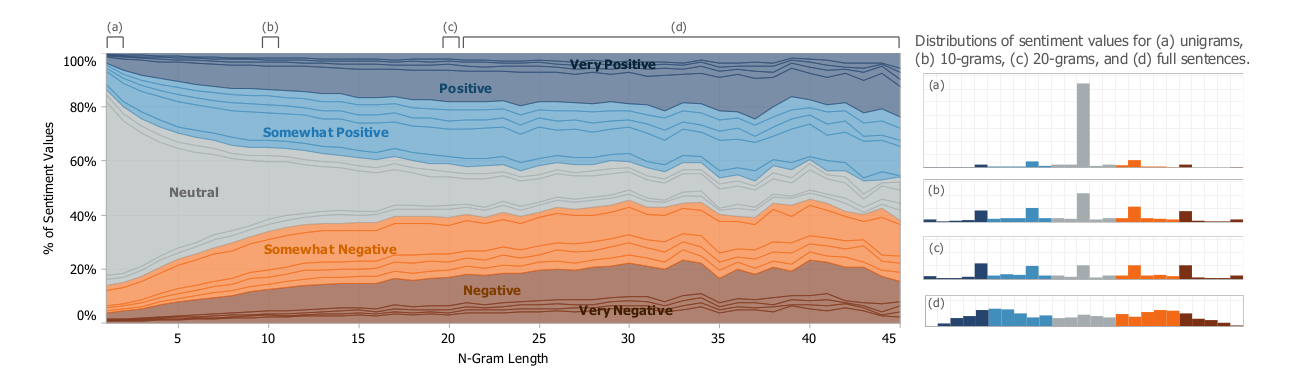
\includegraphics[width=\textwidth]{cropped.png}
\end{figure}

\subsubsection{Recursive Neural Models}
The models in this section compute vectore representations for phrases of variable length and syntactic type. These representations will be then used to classify each phrase. 

When an $n$-gram is given to the compositional models, it is parsed into a binary tree, and each leaf node, corresponding to a word, is represented as a vector. Recursive Neural Models (RNMs) then compute the parent vector in a bottom-up fashion using different types of compositionality functions $g$.

Each word is represented as a $d$-dimensional vector. We initialised all word vectors by randomly sampling each value from a uniform distribution: $\mathcal{U} (-r, r)$ where $r = 0.0001$. All word vectors are stacked in the word embedding matrix $L \in \mathbb{R}^{d \times |V|}$, where $|V|$ is the size of the vocabulary. Initially, the word vectors will be random but the $L$ matrix is seen as a paramater that is trained jointly with the compositionality models.

\begin{figure}[H]
\centering
\caption{Approach of Recursive Neural Network models for sentiment}
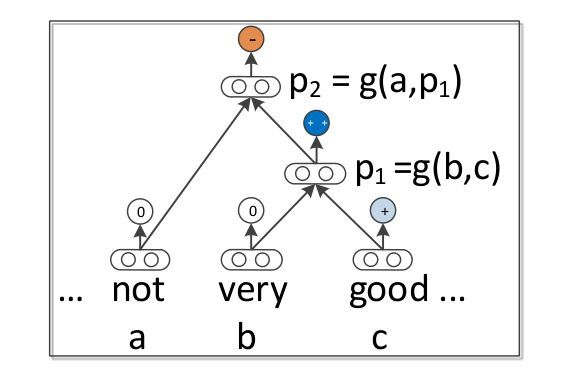
\includegraphics[width=0.5\textwidth]{RNN.png}
\end{figure}

\subsubsection{Recursive Neural Networks}
n the above tree ex-
ample, p1 has its two children’s vectors since both
are words. RNNs use the following equations to
compute the parent vectors:

$$
p_1 = f \Bigg( W \begin{bmatrix}
       b \\[0.3em]
       c \\[0.3em]
     \end{bmatrix} \Bigg), \ p_2 =  \Bigg( W \begin{bmatrix}
       a \\[0.3em]
       p_1 \\[0.3em]
     \end{bmatrix} \Bigg)
$$
where $f = tanh$ is a standard element-wise nonlinearity, $W \in \mathbb{R}^{d \times 2d}$ is the main parameter to learn and we omit the bias for simplicity.

\section{Software/Libraries Used}

\subsection{Stream Processing}

\subsubsection{Apache Storm}
Apache Storm is a free and open source project licensed under the Apache License, Version 2.0, currently undergoing incubation at The Apache Software Foundation (ASF), sponsored by the Apache Incubator

\subsubsection{Twitter4J}
Twitter4J is released under Apache License 2.0.

\subsubsection{Apache Commons}
All packages produced by the ASF are implicitly licensed under the Apache License, Version 2.0, unless otherwise explicitly stated.

\subsection{Sentiment Analysis}
\subsubsection{SenticNet}
SenticNet is an initiative conceived at the MIT Media Laboratory in 2009 within an industrial Cooperative Awards in Science and Engineering (CASE) research project born from the collaboration between the Media Lab, the University of Stirling, and Sitekit Solutions Ltd.

\subsubsection{Stanford CoreNLP}
The Stanford CoreNLP code is written in Java and licensed under the GNU General Public License (v2 or later). Source is included. Note that this is the full GPL, which allows many free uses, but not its use in distributed proprietary software.

\section{Future Work}

\subsection{Product \& Movie Reviews}
Most feature film rating websites like \textbf{rottentomatoes.com} and \textbf{imdb.com} rely on the user to submit a rating to a movie he or she watched, even after writing a review on it. This can be automated using Sentiment Analysis of the review.

\subsection{Personal Assistants}
Personal Assistants like \textbf{Google Now}, \textbf{Siri} and \textbf{Cortana} use Natural Language Processing to a great extent. But in these scenarios, NLP is limited to getting tasks like sending an email, browsing the web, setting alarms etc. So, to develop a much more personalised personal assistant, it needs to \emph{know} the user better. Sentiment analysis of the interaction between the user and the software can foster this notion.

\begin{thebibliography}{9}

\bibitem{stanford}
  Socher, Perelygin et. al., \emph{Recursive Deep Models for Semantic Compositionality Over a Sentiment Treebank}. 
  Stanford University, Stanford.
  
\bibitem{turney}
  Peter D. Turney, \emph{Thumbs Up or Thumbs Down? Semantic Orientation Applied to Unsupervised Classification of Reviews}. 
  Institute for Information Technology, National Research Council of Canada, Canada.  
  
\bibitem{chang}
  Leung \& Chan, \emph{Sentiment Analysis of Product Reviews}. 
  Department of Computing, The Hong Kong Polytechnic University, Hong Kong SAR.

\bibitem{senticnet}
  Erik Cambria, Daniel Olsher \& Dheeraj Rajagopal, \emph{A Common and Common-Sense Knowledge Base
for Cognition-Driven Sentiment Analysis}.

\end{thebibliography}


\end{document}

